% Describe mixedband
In term of compressibility,  people attempt to downsample the signals (e.g., audio waveform, images, etc.) and filter them with a complement of low- and high-pass filters to compact the information into a sparse representation. 
The new low coefficients form another level of detail of that image. 
Hence, successively processing this one until we reach the final delineation will establish a structure of multi-resolution analysis of signals. 
Fig.~\ref{fig:barbara_tradition} shows a grayscale image and one-, two-, three-level of wavelet decomposition using the simplest filters: Haar family. 
The wavelet coefficients have been mapped onto jet color space which indicates the low value coefficients are blue and the high ones are red. 
If the image has been altered by some noise-like impacts, it will result in the high band of wavelet coefficients contain more non-zero values.



\begin{figure}[t]
	\centering  
	%%%%%%%%%%%%%%%%%%%%%%%%%%%%%%%%%%%%%%%%%%%%%%%%%%%%%%%%%%%%%%%%%%%%%%%
	\subfloat[]
    {  
  		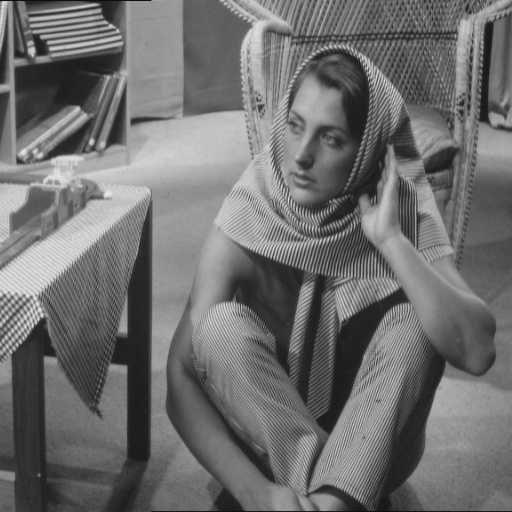
\includegraphics[width=0.3\linewidth]{fig/barbara_gray.png}
	}	\\
    \subfloat[]
    {
		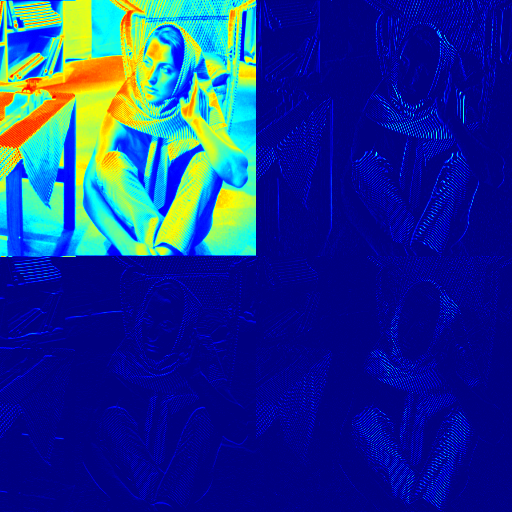
\includegraphics[width=0.3\linewidth]{fig/barbara_tradition_1.png}
    }	
	\subfloat[]
    {  
  		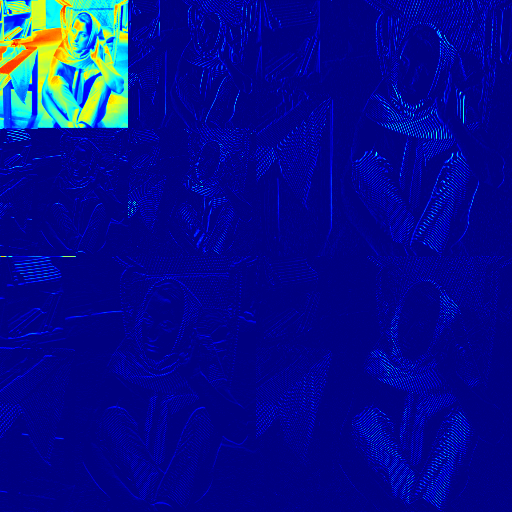
\includegraphics[width=0.3\linewidth]{fig/barbara_tradition_2.png}
	}	
		\subfloat[]
    {  
  		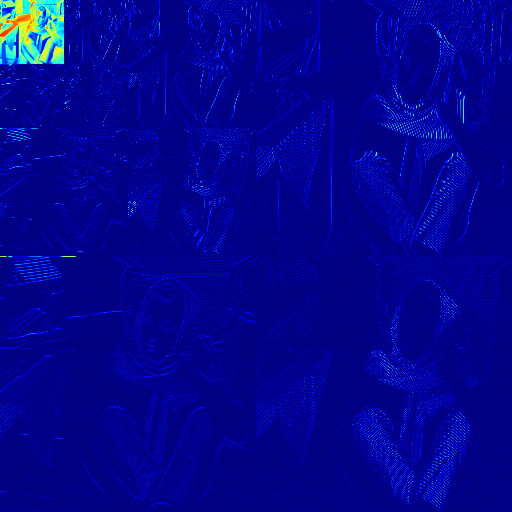
\includegraphics[width=0.3\linewidth]{fig/barbara_tradition_3.png}
	}	\\
\caption{TODO}
\label{fig:barbara_tradition}
\end{figure}



% Describe usefulness
In this paper, we describe straightforward techniques to speedup DWT on the GPU. 
It can be further extended to be embedded into other methods such as combining with Split-Bregman algorithm~\cite{goldstein_split_2009} in 3D Compressive Sensing (CS) MRI  reconstruction, performing many-step image reconstruction by iteratively solving an inverse problem and so on. 
Without going deeply into those mentioned approaches, we bring several advantage features that mixed-band wavelet can be more useful.

% Structure of the paper
The rest of the paper is organized as follows. First, we briefly explain the historical directions of signal analysis as well as data compression and the current state of discrete wavelet transform on this domain in the next.
Second, we describe several ways to deal with the advantages which mixed-band wavelet brings back and how to implement those on the GPU with Compute Unified Device Architecture (CUDA)~\cite{CUDA} programming model.
Third, the performance of traditional wavelet and mixed-band wavelet transform are also measured on either CPU or GPU side to see how benefit we can gain by interleaving wavelet bands on the memory layout.
We also discuss the roll of DWT in 3D CSMRI reconstruction to exploit the  
We conclude our work in the last section, discuss pros and cons and then further suggest some future works in this direction.

